\chapter{Results}\label{ch:results}

All server runs have finished. FISTA has been rescored at matching depths, and FISTA-Net has been rerun.

\section{The main table}

All numbers are mean errors. Lower is better.

\begin{center}
\small
\begin{tabular}{lccc}
\toprule
Method & Simulated validation & COMSOL (15 pairs) & COMSOL NRMSE \\
\midrule
ISTA, 16 iterations & 64.3\% & 64.4\% & 4.60\% \\
Wiener & 60.3\% & 49.3\% & 3.53\% \\
Eq.~20, sparse, relative, 16 layers & 45.6\% & 42.0\% & 3.01\% \\
FISTA-32, $\lambda=0.03$ & 50.9\% & 41.8\% & 3.00\% \\
Eq.~20, sparse, MSE, 16 layers & 48.6\% & 40.2\% & 2.88\% \\
FISTA-Net run 1 & 65.2\% & 39.4\% & 2.85\% \\
Eq.~20, plain, MSE, 16 layers & 53.4\% & 39.1\% & 2.80\% \\
Eq.~20, sparse, relative, 32 layers & 42.5\% & 38.9\% & 2.80\% \\
FISTA-64, $\lambda=0.009$ & 45.3\% & 37.9\% & 2.72\% \\
Eq.~20, strict, 32 layers & 51.9\% & 35.4\% & 2.54\% \\
LFISTA-style, 32 layers & 42.8\% & 34.2\% & 2.47\% \\
Eq.~20, strict, 64 layers & 48.8\% & 33.8\% & 2.43\% \\
\textbf{FISTA-Net run 2} & \textbf{47.9\%} & \textbf{33.3\%} & \textbf{2.41\%} \\
FISTA-300, $\lambda=0.03$ & 36.6\% & 32.1\% & 2.33\% \\
\textbf{FISTA-300, $\lambda=0.009$} & \textbf{35.5\%} & \textbf{30.5\%} & \textbf{2.20\%} \\
\bottomrule
\end{tabular}
\end{center}

\begin{figure}[H]
\centering
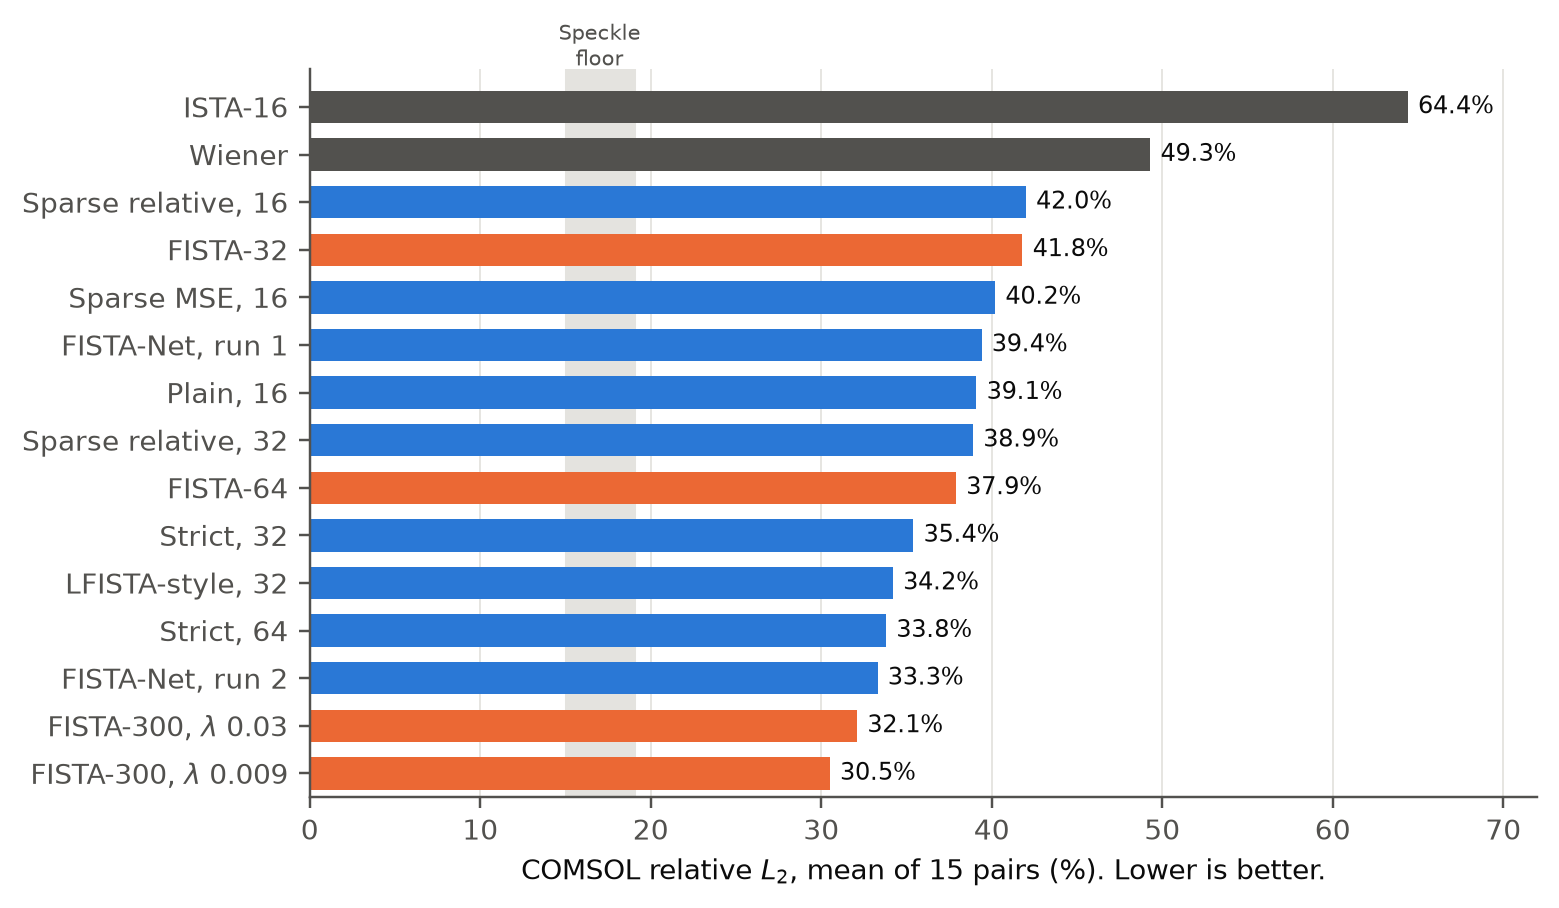
\includegraphics[width=\textwidth]{results}
\caption{The COMSOL scores from the table. Grey bars are simple baselines, blue bars are trained networks, and
orange bars are FISTA with the same dictionary and no trained layers. The shaded band is the speckle floor
from Chapter~\ref{ch:simulation}.}
\label{fig:results}
\end{figure}

\begin{keyidea}[The current picture]
\begin{itemize}
\item \textbf{Best overall:} FISTA-300 at 30.5\%, a classical method using the learned dictionary.
\item \textbf{Selected network:} FISTA-Net run 2, 33.3\%. Among the runs without our floor and loss changes, it has the
lowest simulated validation error, so this choice does not use COMSOL.
\item \textbf{Close behind:} strict Eq.~20 at 64 layers, 33.8\%, and the LFISTA-style network, 34.2\%. All three networks sit
within 1 point, which is too small to rank on one seed each.
\end{itemize}
\end{keyidea}

\section{Networks against FISTA at equal depth}

This is the fair way to ask whether learning helped. One layer and one FISTA iteration do similar work, so
compare them at the same count.

\begin{center}
\begin{tabular}{rcccc}
\toprule
& \multicolumn{2}{c}{COMSOL} & \multicolumn{2}{c}{Simulated validation} \\
Depth & FISTA & Strict Eq.~20 & FISTA & Strict Eq.~20 \\
\midrule
32 & 41.8\% & \textbf{35.4\%} & \textbf{50.9\%} & 51.9\% \\
64 & 37.9\% & \textbf{33.8\%} & 45.3\% & 48.8\% \\
300 & 30.5\% & Not trained & 35.5\% & Not trained \\
\bottomrule
\end{tabular}
\end{center}

\begin{figure}[H]
\centering
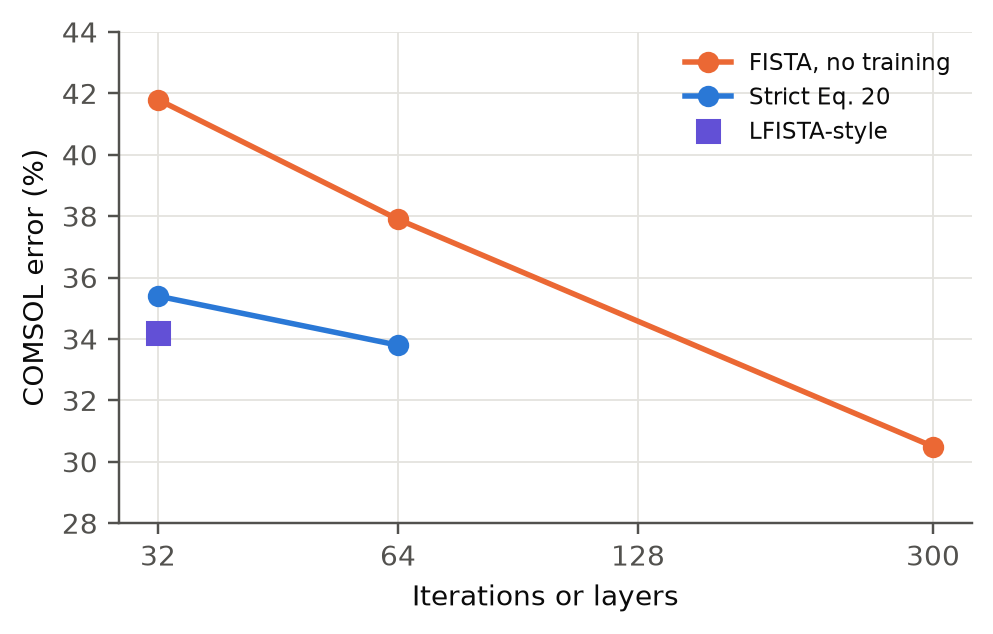
\includegraphics[width=.68\textwidth]{depth}
\caption{COMSOL error against depth. At 32 and 64 steps the networks win. FISTA keeps improving with more
iterations and passes them by 300. Note the log scale.}
\label{fig:depth}
\end{figure}

So on COMSOL, learning gives a gain of about 6 points at 32 layers and 4 at 64. On simulated validation, the same
networks \emph{lose} to FISTA at the same depth, by 1 and 3.5 points. The gain appears only on COMSOL, and we do not
know why. It is worth being careful about this before claiming it as a win.

\begin{careful}[No speed claim yet]
It is tempting to say that 64 layers do the work of about 300 iterations, but that is not what the data shows, since
64 layers do not reach FISTA-300's score. Also, run time was never measured. So there is no speed advantage you can claim
yet.
\end{careful}

\section{How FISTA's $\lambda$ was retuned}

The first version of this booklet warned that $\lambda=0.03$ sat at the edge of the search grid. So FISTA was rescored per
depth with \code{scripts/score_fista_depths.py}, on a wider grid. Each $\lambda$ was again chosen on the first 16
simulated validation crops only.

\begin{center}
\begin{tabular}{ccccccccc}
\toprule
$\lambda$ & 7e-7 & 0.0003 & 0.003 & 0.009 & 0.03 & 0.09 & 0.3 & 0.9 \\
\midrule
FISTA-300 on 16 crops & 40.0\% & 36.1\% & 24.4\% & \textbf{22.4\%} & 24.5\% & 29.4\% & 41.3\% & 55.3\% \\
\bottomrule
\end{tabular}
\end{center}

Now the best value sits inside the grid, with worse values on both sides. The chosen values are 0.03 for FISTA-32 and
0.009 for FISTA-64 and FISTA-300. The old $\lambda=0.03$ score reproduced exactly, at 32.1\%, which confirms that the new
script and the first run agree.

\begin{careful}[FISTA-64's $\lambda$ is uncertain]
The 16 crops chose 0.009, but on all 64 crops 0.03 was slightly better, 44.9\% against 45.3\%. Both give about 38\% on
COMSOL, so it barely matters here, but 16 crops is a small sample.
\end{careful}

\section{By component and configuration}

\begin{center}
\begin{tabular}{lccc}
\toprule
Mean over 5 configurations & $B_x$ & $B_y$ & $B_z$ \\
\midrule
Wiener & 47.7\% & 48.1\% & 52.2\% \\
FISTA-32 & 40.0\% & 40.2\% & 45.2\% \\
FISTA-Net run 1 & 36.2\% & 36.2\% & 46.0\% \\
FISTA-64, $\lambda=0.009$ & 36.2\% & 36.4\% & 41.2\% \\
Strict, 32 layers & 33.6\% & 33.6\% & 39.1\% \\
LFISTA-style, 32 layers & 32.8\% & 31.4\% & 38.5\% \\
FISTA-Net run 2 & 30.2\% & 30.7\% & 39.1\% \\
Strict, 64 layers & 31.8\% & 32.0\% & 37.5\% \\
FISTA-300, $\lambda=0.009$ & 29.0\% & 27.8\% & 34.7\% \\
\bottomrule
\end{tabular}
\end{center}

$B_z$ is always the hardest. This matches the simulator, which also has its largest error on $B_z$, and the speckle,
which is strongest there.

\begin{center}
\begin{tabular}{lccccc}
\toprule
Mean over 3 components & L1\_C1 & IC\_4um & C1+C2 & C1+C2+C3 & C1--C4 \\
\midrule
Wiener & 49.3\% & 50.1\% & 49.1\% & 49.0\% & 49.0\% \\
FISTA-32 & 41.2\% & 45.0\% & 41.0\% & 40.9\% & 41.0\% \\
FISTA-Net run 1 & 39.0\% & 42.1\% & 38.9\% & 38.7\% & 38.5\% \\
FISTA-Net run 2 & 33.1\% & 34.6\% & 33.2\% & 33.1\% & 32.7\% \\
FISTA-64, $\lambda=0.009$ & 38.3\% & 36.9\% & 38.2\% & 38.1\% & 38.1\% \\
Strict, 32 layers & 36.3\% & 32.3\% & 36.3\% & 36.1\% & 36.1\% \\
LFISTA-style, 32 layers & 35.3\% & 30.1\% & 35.3\% & 35.2\% & 35.2\% \\
Strict, 64 layers & 34.6\% & 30.7\% & 34.6\% & 34.5\% & 34.5\% \\
FISTA-300, $\lambda=0.009$ & 31.2\% & 27.6\% & 31.4\% & 31.2\% & 31.1\% \\
\bottomrule
\end{tabular}
\end{center}

Four of the five columns are nearly equal, because they contain the same wire shape. Only IC\_4um is a different coil. Most
methods do better on it, but FISTA-32 and both FISTA-Net runs do worse. So one extra wire shape can change the ranking, which is
another reason to treat 15 pairs from two shapes with care.

\section{What the outputs look like}

\begin{figure}[H]
\centering
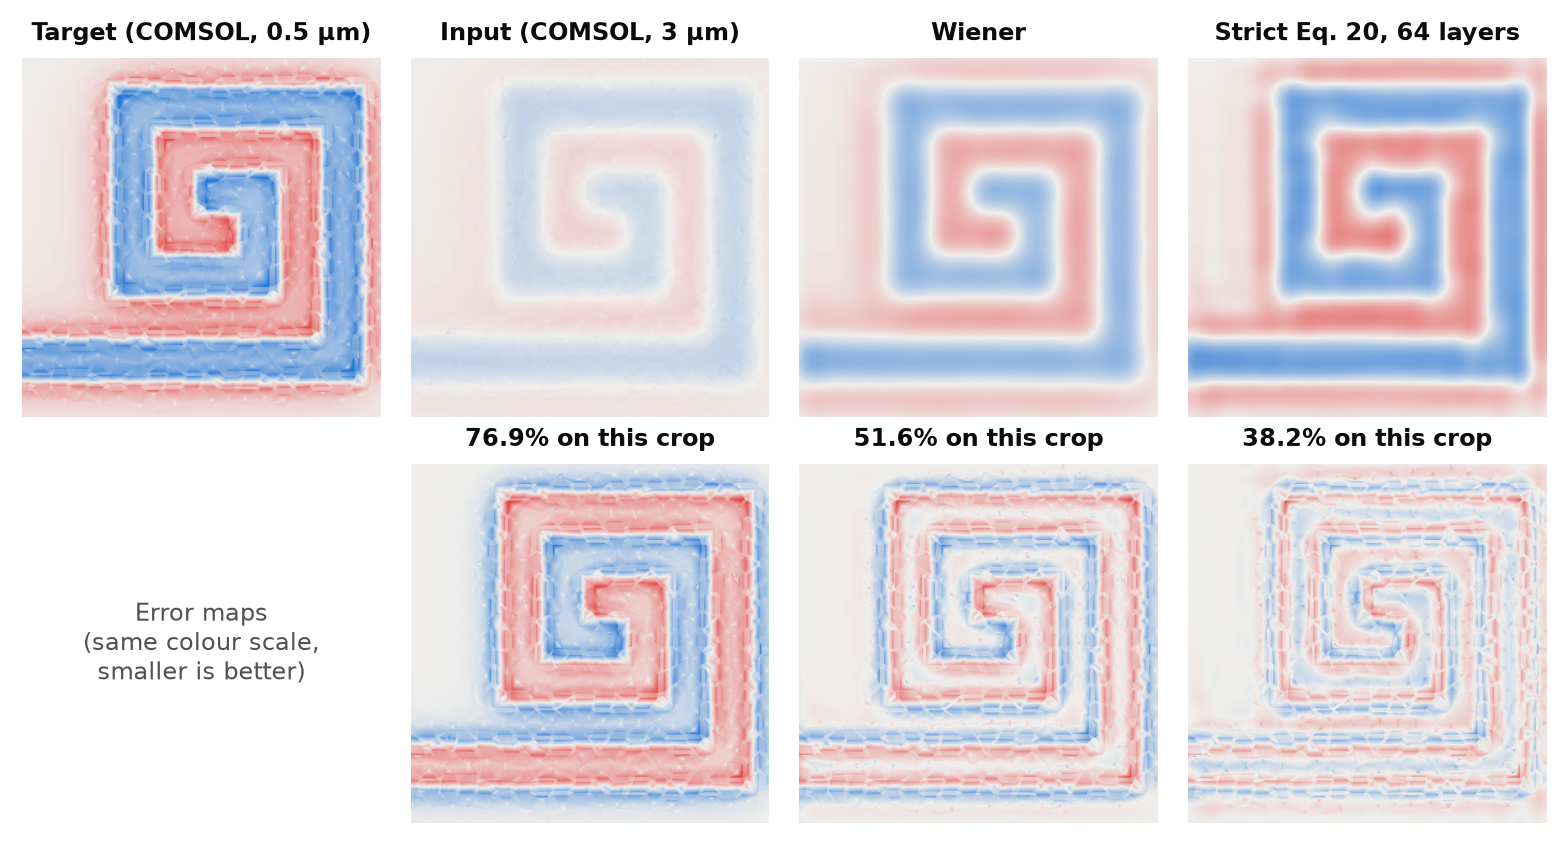
\includegraphics[width=\textwidth]{reconstruction}
\caption{$B_z$ of the COMSOL L1\_C1 coil, on the 512 pixel window with the most signal. The top row shares one colour
scale. The bottom row shows output minus target on that same scale. The output was computed from the zero-padded 512
pixel crop alone, so it is not a cut-out of the full-image prediction, and the percentages apply to this crop only.
Note the fine mesh speckle in the target: no method can or should reproduce it.}
\label{fig:reconstruction}
\end{figure}

Three things are visible in Figure~\ref{fig:reconstruction}.

\begin{enumerate}
\item The input is much too weak, so its error map still looks like the coil.
\item Wiener restores some strength, but its edges stay soft.
\item Strict Eq.~20 is much closer in strength, and its remaining error sits mostly on wire edges.
\end{enumerate}

\begin{figure}[H]
\centering
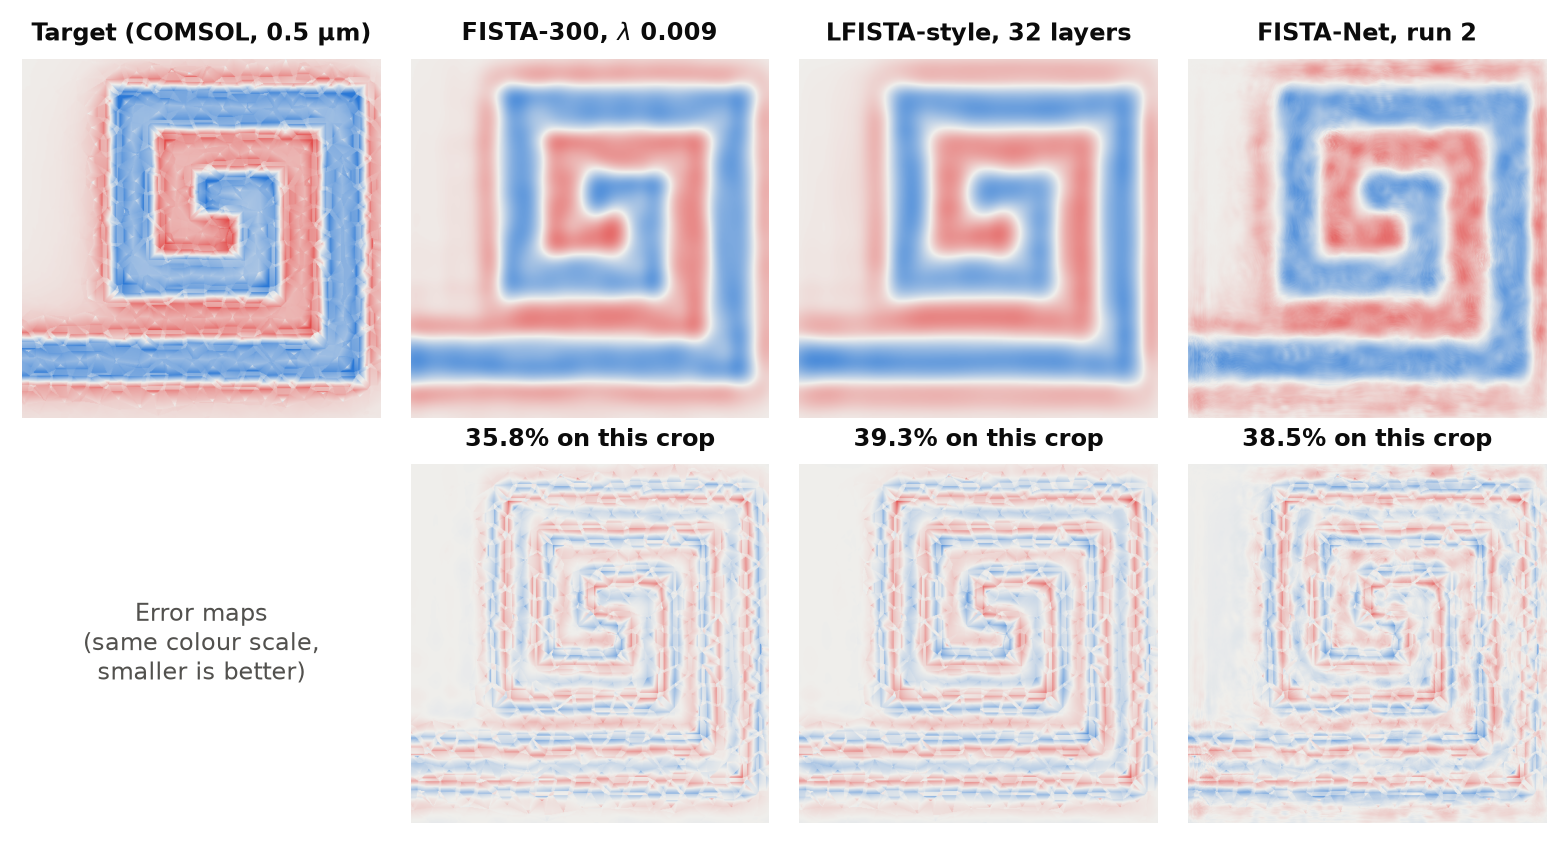
\includegraphics[width=\textwidth]{reconstruction_new}
\caption{The same crop and colour scale for three other methods. Again, the percentages apply to this crop only.}
\label{fig:reconstruction-new}
\end{figure}

\section{Seven honest lessons}

\subsection*{1. Depth helps every method}

Networks: 39.1, 35.4 and 33.8\% at 16, 32 and 64 layers. FISTA: 41.8, 37.9 and 30.5\% at 32, 64 and 300. For the networks,
the gain per doubling is shrinking, and the first of those runs also had a different length.

\subsection*{2. Learning helps at equal depth, but FISTA-300 still wins}

Strict Eq.~20 and the LFISTA-style network beat FISTA at 32 and 64 steps on COMSOL. Nothing trained so far reaches FISTA-300.

\subsection*{3. Simulated validation does not predict COMSOL}

\begin{figure}[H]
\centering
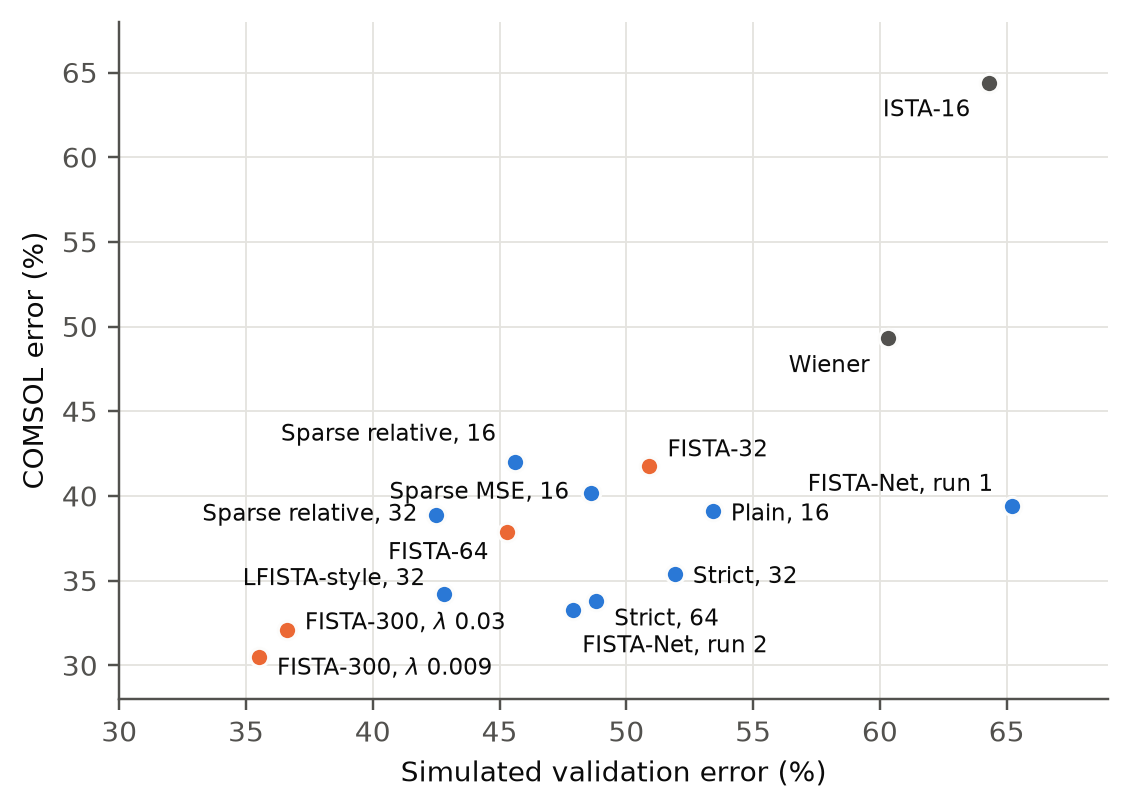
\includegraphics[width=.8\textwidth]{rank}
\caption{Each dot is a method. If simulated validation predicted COMSOL well, the dots would form a tight rising line.
FISTA-Net run 1 is the clearest exception: it has the worst simulated score of all, yet it beats Wiener, ISTA-16 and
FISTA-32 on COMSOL. The sparse 32-layer run also beats the two strict runs on simulation and loses to them on COMSOL.}
\label{fig:rank}
\end{figure}

This is the most important warning in this booklet. We pick checkpoints and settings on simulated validation, because
COMSOL must stay untouched. Yet Figure~\ref{fig:rank} shows that a better simulated score does not reliably give a better
COMSOL score. The simulator is not a perfect copy of COMSOL.

\subsection*{4. Early peaking belongs to the MSE runs}

MSE runs get their best validation score at step 200--300, then get worse. Strict 64 went from 48.8\% at step 200 to 52.3\%
at step 1,000. The LFISTA-style run behaves differently: its validation error improved all the way to the last step. It has
no target in its loss, so it cannot fit the training targets. This is a hint that MSE fitting is part of the problem, but it
is one run of each, and the cause is not established.

\subsection*{5. A sparse network can match a dense one}

The LFISTA-style network keeps its codes 16.6\% dense, and still reaches 34.2\%. So the dense behaviour of strict
Eq.~20 is not required for a good score. See Chapter~\ref{ch:density}.

\subsection*{6. A tiny network can match a huge one}

FISTA-Net has 74,599 parameters, and strict Eq.~20 at 64 layers has 49.2 million, about 660 times more. It also needs no
dictionary. Yet they score about the same. The price was training time: run 2 took about 27 hours, against about 3 for
strict 64 layers.

\subsection*{7. There is a floor}

COMSOL's speckle lies in the target, so no clean method should score below about 15--19\%. From FISTA-300's 30.5\%, that
leaves at most about 12--16 points.

\section{Caveats to state out loud}

\begin{careful}
\begin{itemize}
\item \textbf{Best of many.} After many methods are compared on COMSOL, the best score is a little optimistic, even though
no setting was chosen on COMSOL. If you keep trying methods and report only the winner, you are slowly using the test set.
\item \textbf{FISTA-Net got a second chance.} Run 2 exists because of what run 1 showed, and an interim COMSOL score was read
during run 2. It changed nothing in the run, but no other network was rerun this way.
\item \textbf{A noisy checkpoint.} FISTA-Net's validation error still swings widely, and its best step was picked from 91
checks, so 47.9\% is partly a lucky draw. Its last 300 steps ranged from 47.9\% to 54.3\%.
\item \textbf{The baseline moved.} FISTA was retuned after the COMSOL scores of the networks were known. The $\lambda$ was chosen on
simulated crops only, and the widening was prompted by the grid edge, not by a COMSOL score. Say this openly anyway.
\item \textbf{Unequal tuning.} FISTA got a search over eight $\lambda$ values. The LFISTA-style run still uses
$\lambda=0.03$, and $0.009$ has not been tried for it.
\item \textbf{Two wire shapes.} The 15 pairs are not 15 independent tests.
\item \textbf{One seed.} No error bars exist.
\item \textbf{Prior knowledge.} The generator was designed with these coils in view.
\end{itemize}
\end{careful}
